\documentclass{beamer}
%\documentclass[handout]{beamer}


%%%%%%%%%%%%%
%% THEMES w/o navigaton
%\usetheme{default}
%\usetheme{Madrid}
%\usetheme{Pittsburgh}
\usetheme{Boadilla}

%%%%%%%%%%%%%
%% THEMES w/ tree navigation
%\usetheme{Antibes}

%%%%%%%%%%%%%
%% THEMES w/ TOC sidebar
%\usetheme{Berkeley}
%\usetheme{PaloAlto}


%%%%%%%%%%%%%
%% THEMES w/ miniframe navigation
%\usetheme{Berlin}
%\usetheme{Darmstadt}
%\usetheme{Ilmenau}
%\usetheme{Singapore}
%\usetheme{Frankfurt}

%%%%%%%%%%%%%
%% THEMES w/ section/subsection titles
%\usetheme{Copenhagen}
%\usetheme{Warsaw}





%% COLOR THEMES %%
%\usecolortheme{dove}
%\usecolortheme{beaver}


%%%%%%%%%%%%%%%

\usepackage{multirow}

\usepackage{tikz}
\usetikzlibrary{arrows}

\DeclareMathOperator*{\argmax}{arg\,max}
\DeclareMathOperator*{\argmin}{arg\,min}
%\DeclareMathOperator*{\Em}{E_w(x=x^{(m)},h)}
\DeclareMathOperator*{\Em}{E_w(x^{(m)},h)}
\DeclareMathOperator*{\E}{E_w(x,h)}
\DeclareMathOperator*{\Es}{E(x,h)}
%\DeclareMathOperator*{\nw}{\nabla_{w_{ij}}}
\DeclareMathOperator*{\nw}{\partial_{w_{ij}}}
\newcommand{\btheta}{\boldsymbol \theta }
\newcommand{\bi}{\begin{itemize}}
\newcommand{\ei}{\end{itemize}}
\newcommand{\be}{\begin{enumerate}}
\newcommand{\ee}{\end{enumerate}}


%\setbeamertemplate{footline}{\hfill\insertframenumber/\inserttotalframenumber}

\setbeamertemplate{footline}[text line]{%
  \parbox{\linewidth}{\hfill (p.\insertframenumber})}
\setbeamertemplate{navigation symbols}{}


\setbeamertemplate{bibliography item}{}


\makeatletter
\def\blfootnote{\xdef\@thefnmark{}\@footnotetext}
\makeatother

\makeatother


\title{Representation Learning for Text}
\author{Kevin Duh}
\institute{Johns Hopkins University}
\date{June 2017}


\AtBeginSubsection[]
{
  \begin{frame}
    \small{\frametitle{Outline}
    \tableofcontents[currentsection,currentsubsection]
	}
  \end{frame}
}
\AtBeginSection[]
{
  \begin{frame}
    \small{\frametitle{Outline}
    \tableofcontents[currentsection,currentsubsection]
	}
  \end{frame}
}

\begin{document}

\begin{frame}
\titlepage
\end{frame}

%%%%%%%%%%%%%
\begin{frame}
\frametitle{Terminology}
\bi 
\item Representation Learning is a problem statement
\item Deep Learning is a solution technique
\item Neural network is a way of implementing deep learning
\ei
\centerline{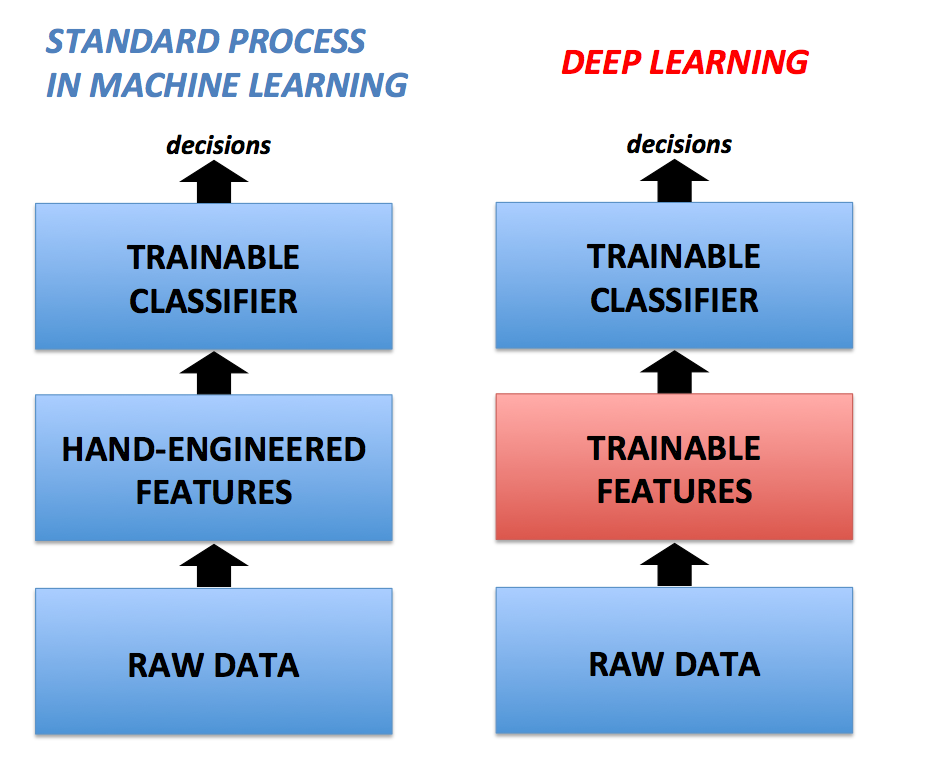
\includegraphics[scale=0.25]{figs/deep_vs_conventional_learning}}
\end{frame}


\begin{frame}
\frametitle{Representation Learning in Images}
Automatically trained features make sense! \cite{lee09convolutional}\\[0.2cm]
Input: Images (raw pixels)\\
$\rightarrow$ Output: Features of Edges, Body Parts, Full Faces

\centerline{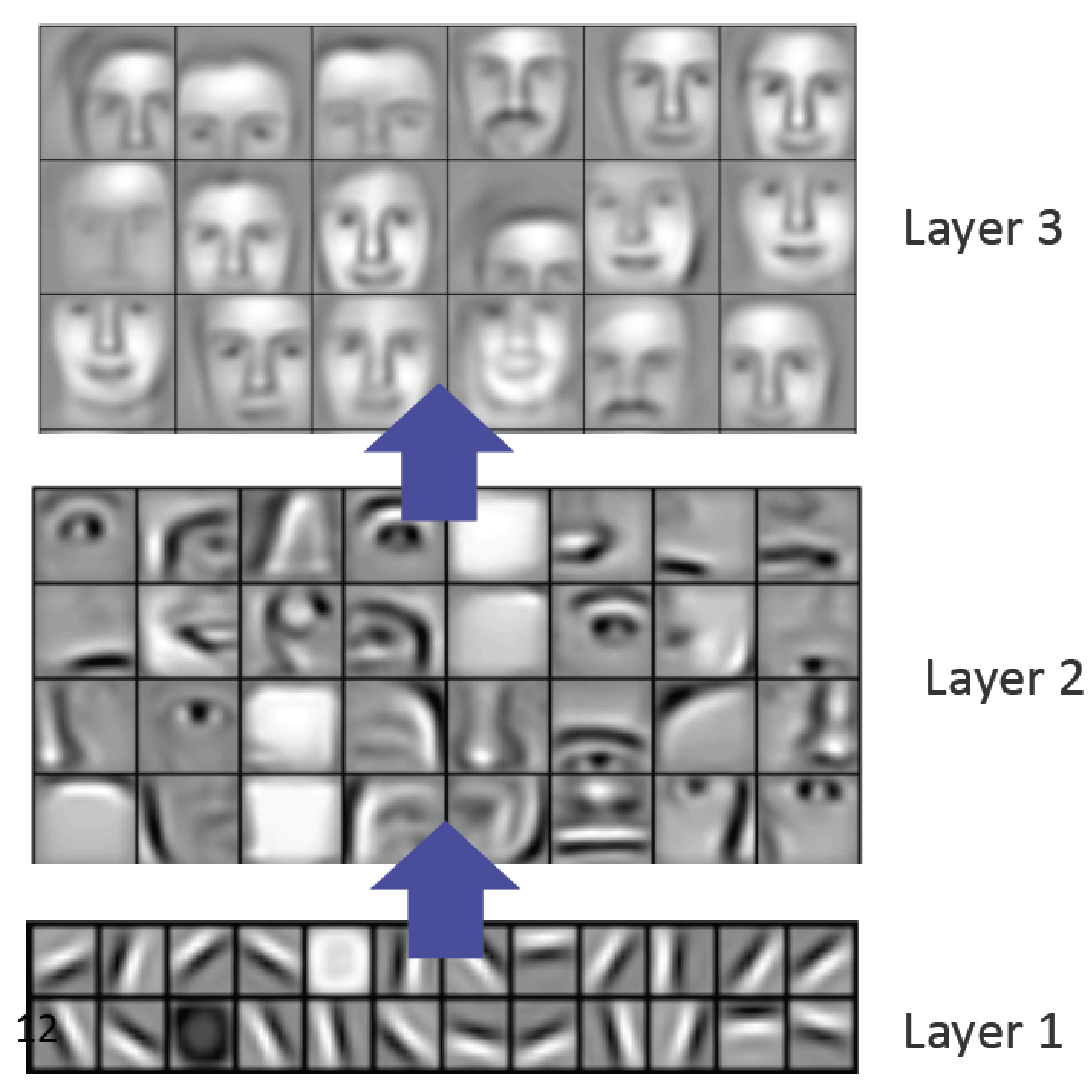
\includegraphics[scale=0.35]{figs/lee09example}}
\end{frame}

\begin{frame}
\small{\frametitle{Outline}
\tableofcontents
}
\end{frame}

%% SECTION%%%%%
\section[Word Embedding]{Word Embeddings}

%%% subection
\subsection[What to represent]{What should be encoded in a word representation?}

\begin{frame}
\frametitle{Representations of Words}
\bi
\item Central question: How to computationally represent ``words'' in a natural language processing system? 
\begin{figure}[htbp]
\begin{center}
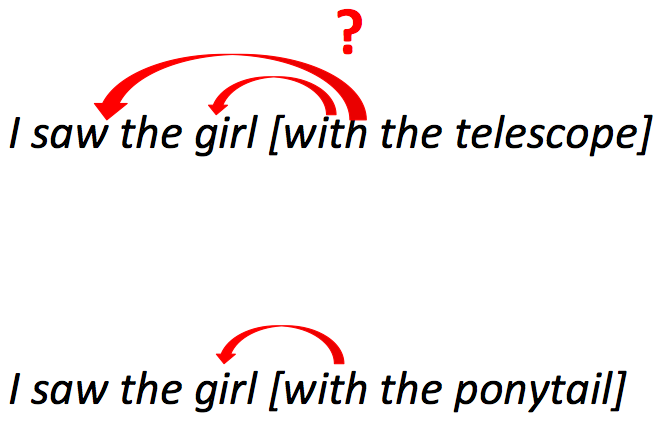
\includegraphics[width=0.6\textwidth]{figs/sentence_ambiguity}
\end{center}
\end{figure}
\ei
\end{frame}


\begin{frame}
\frametitle{Vector Representation of Words (word embeddings)}
\begin{itemize}
\item Embed word in vector space, such that nearby words are syntactically or semantically similar
\item Neural nets can be used to learn these vectors from raw text \cite{collobert11scratch,chen13embedding}
\end{itemize}
\centerline{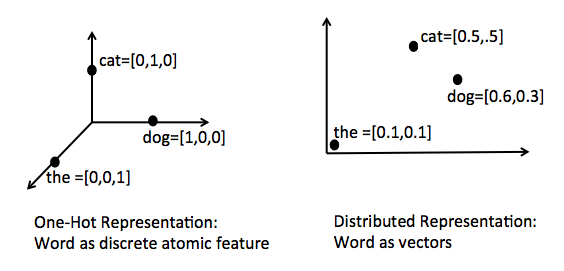
\includegraphics[scale=0.5]{figs/onehot_vs_embedding}}
\end{frame}


\begin{frame}
\frametitle{Vector Representations of Words (Word Embeddings)}
\begin{figure}[htbp]
\begin{center}
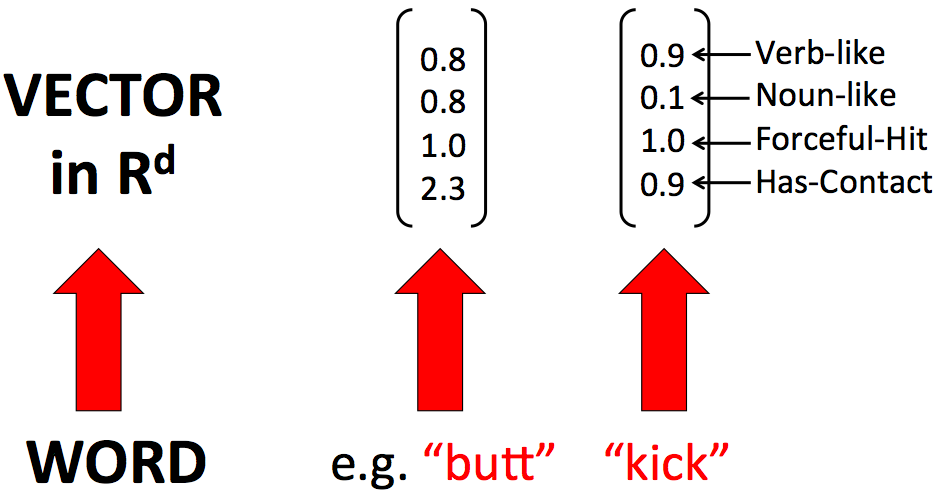
\includegraphics[width=0.9\textwidth]{figs/word_embedding1}
\end{center}
\end{figure}
\end{frame}

\begin{frame}
\frametitle{Vector Representations of Words (Word Embeddings)}
\begin{figure}[htbp]
\begin{center}
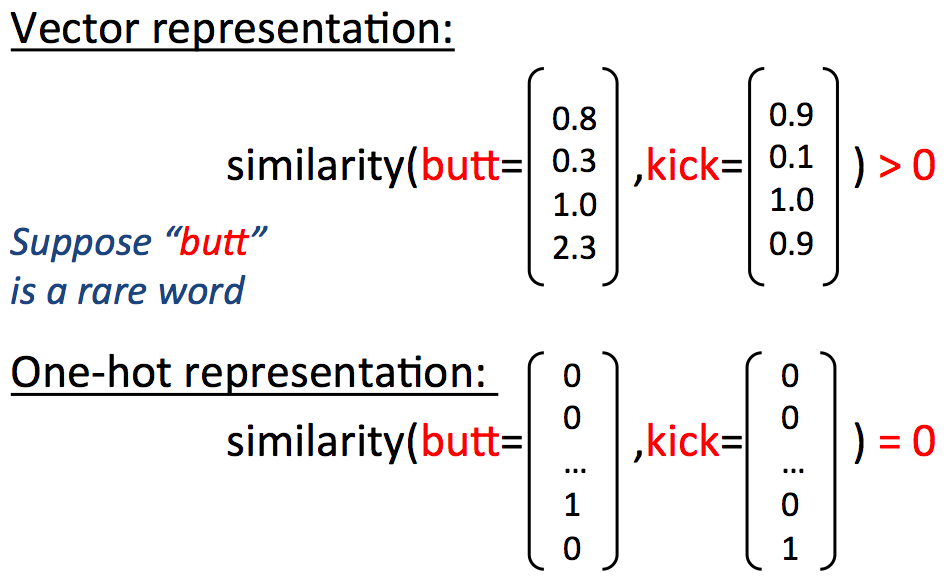
\includegraphics[width=0.9\textwidth]{figs/word_embedding2}
\end{center}
\end{figure}
\end{frame}

\begin{frame}
\frametitle{What information is needed for a good representation?}
\begin{figure}[htbp]
\begin{center}
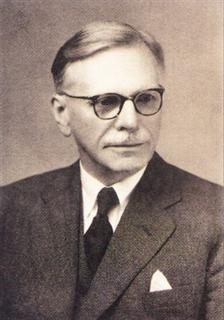
\includegraphics[width=0.3\textwidth]{figs/john_firth}
\end{center}
\end{figure}
You shall know a word by the company it keeps. -- J. R. Firth (linguist)
\bi
\item Distributional Semantics: a word's meaning is based on its positional distribution in text
\ei
\end{frame}

\begin{frame}
\frametitle{Distributional Semantics}
\begin{figure}[htbp]
\begin{center}
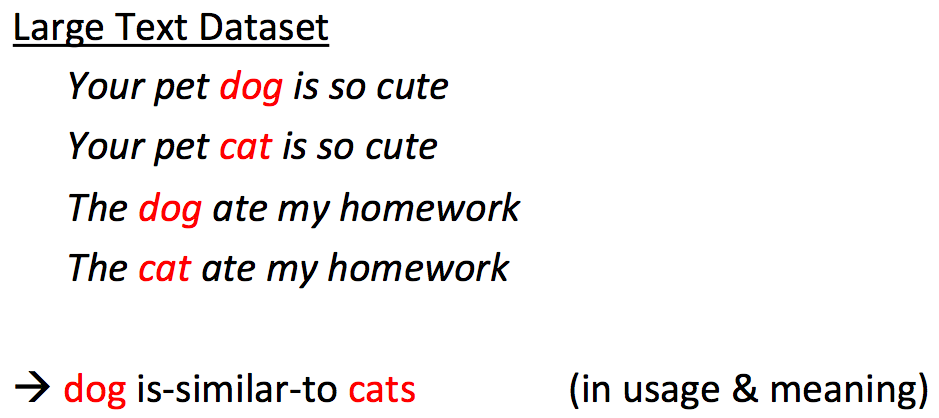
\includegraphics[width=0.9\textwidth]{figs/distributional_semantics_example}
\end{center}
\end{figure}
\end{frame}

\begin{frame}
\frametitle{Example: "Bar-ba-loots"}
\bi
\item Do you know what is a bar-ba-loot?
\pause
\item Which has higher probability?
	\bi 
	\item $P(\mathbf{w_t}=fruits \mid \mathbf{w_{t-1}}=like, \mathbf{w_{t-2}}=Bar\mbox{-}ba\mbox{-}loots)$
	\item $P(\mathbf{w_t}=looting\hspace{0.16cm} \mid \mathbf{w_{t-1}}=like, \mathbf{w_{t-2}}=Bar\mbox{-}ba\mbox{-}loots)$
	\ei
\pause
\item What if I tell you \textbf{vector}(Bar-ba-loots) $\sim$ \textbf{vector}(bears)?
\centerline{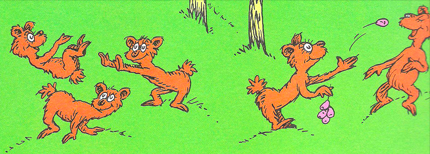
\includegraphics[scale=0.5]{figs/bar_ba_loots}}
\pause
\item Purpose of word embedding: Improve generalization
\ei

\end{frame}

%%% subsection
\subsection{Neural language model and word2vec}

\begin{frame}
\frametitle{Neural language model and word2vec}
\bi
\item Feed-forward neural language model 
	\bi
	\item Model $P(\mathbf{w_t}=looting\hspace{0.16cm} \mid \mathbf{w_{t-1}}=like, \mathbf{w_{t-2}}=Bar\mbox{-}ba\mbox{-}loots)$ with a feed-forward neural LM
	\item Can be used a LM inside machine translation / speech recognition systems
	\item Or, can extract first layer as word embedding
	\ei
\item word2vec
	\bi
	\item If we only want word embeddings and don't need a probability distribution over next words, we can save on training time
	\ei
\ei
\end{frame}

\begin{frame}
\frametitle{Word embeddings from Neural LM, one method \begin{small}\cite{bengio03neurallm}\end{small}}
\begin{columns}
\column{0.8\textwidth}
\scalebox{0.8}{\begin{tikzpicture}[->,>=stealth',shorten >=1pt,auto,node distance=3cm,
  thick,main node/.style={circle,fill=blue!20,draw,font=\sffamily\Large\bfseries}]

  \node[main node] (x1) at (0,-3) {$x_1$};
  \node[main node] (x2) at (2,-3) {$x_2$};
  \node[main node] (x3) at (4,-3) {$x_3$};
  \node[main node] (x4) at (6,-3) {$x_4$};
  \node[main node] (x5) at (8,-3) {$x_5$};
  \node[main node] (x6) at (10,-3) {$x_6$};

  \node[main node] (v1) at (1,0) {$v_1$};
  \node[main node] (v2) at (3,0) {$v_2$};
  \node[main node] (v3) at (7,0) {$v_3$};
  \node[main node] (v4) at (9,0) {$v_4$};

  \node[main node] (h1) at (3,2) {$h_1$};
  \node[main node] (h2) at (5,2) {$h_2$};
  \node[main node] (h3) at (7,2) {$h_3$};

  \node[main node] (y1) at (3,4) {$y_1$};
  \node[main node] (y2) at (5,4) {$y_2$};
  \node[main node] (y3) at (7,4) {$y_3$};


  \draw[blue,ultra thick,-latex,<->] (0,-4) -- node[]{Word at t-2, $[x_1,x_2,x_3]=[0,1,0]$} (4,-4);
  \draw[blue,ultra thick,-latex,<->] (0,-1.5) -- node[]{Distributed representation} (4,-1.5);
 \draw[blue,ultra thick,-latex,<->] (6,-4) -- node[]{Word at t-1, $[x_4,x_5,x_6]=[1,0,0]$} (10,-4);
 \draw[blue,ultra thick,-latex,<->] (6,-1.5) -- node[]{Distributed representation} (10,-1.5);
  \draw[blue,ultra thick,-latex,<->] (3,4.6) -- node[]{$P(current\_word=k)=y_k=\frac{\exp(W_{jk}^T h)}{\sum_{k'}\exp(W_{jk'}^T h)}$} (7,4.6);

   \node(co) at (10,2) {Compression: $h=\sigma(M^T v)$};
   \node(M) at (1,1) {$M$};
   \node(wjk) at (1,3) {$w_{jk}$};
      \node(wij) at (3,-2) {$w_{ij}$};

  \path[every node/.style={font=\sffamily\small}]
    (x1) edge node {} (v1)
    (x1) edge node {} (v2)
    (x2) edge node {} (v1)
    (x2) edge node {} (v2)
    (x3) edge node {} (v1)
    (x3) edge node {} (v2)
    (x4) edge node {} (v3)
    (x4) edge node {} (v4)
    (x5) edge node {} (v3)
    (x5) edge node {} (v4)
    (x6) edge node {} (v3)
    (x6) edge node {} (v4)

    (v1) edge node {} (h1)
    (v2) edge node {} (h1)
    (v3) edge node {} (h1)
    (v4) edge node {} (h1)
    (v1) edge node {} (h2)
    (v2) edge node {} (h2)
    (v3) edge node {} (h2)
    (v4) edge node {} (h2)
    (v1) edge node {} (h3)
    (v2) edge node {} (h3)
    (v3) edge node {} (h3)
    (v4) edge node {} (h3)
    
    (h1) edge node {} (y1)
    (h2) edge node {} (y1)
    (h3) edge node {} (y1)
    (h1) edge node {} (y2)
    (h2) edge node {} (y2)
    (h3) edge node {} (y2)
    (h1) edge node {} (y3)
    (h2) edge node {} (y3)
    (h3) edge node {} (y3)
    ;
\end{tikzpicture}}
\column{.2\textwidth}
\end{columns}
\end{frame}

\begin{frame}
\frametitle{Training a Neural LM}
\bi
\item Find parameters $\theta$ that maximizes likelihood $P_{\theta}(\mathbf{w_t} \mid \mathbf{w_{t-1}}, \mathbf{w_{t-2}})$ on training data
	\bi
	\item For each input $\mathbf{x_{t}} = (\mathbf{w_{t-1}}, \mathbf{w_{t-2}})$ and output $\mathbf{w_t} $ pair, forward compute $P_\theta(\cdot)$ and then back-prop 
	\ei
\pause
\item $P_{\theta}(\mathbf{w_t} \mid \mathbf{x_{t}}) = softmax(score(\mathbf{w_t} , \mathbf{x_{t}})) = \frac{ \exp(score(\mathbf{w_t} , \mathbf{h_{t}})) }{\sum_{\mathbf{w'}  \in Vocabulary} \exp(score(\mathbf{w'} , \mathbf{x_{t}))}   }$
\item max-likelihood objective: $\log P_{\theta}(\mathbf{w_t} \mid \mathbf{x_{t}})  = score(\mathbf{w_t} , \mathbf{x_{t}}) - \log \sum_{\mathbf{w'}  \in Vocabulary} \exp(score(\mathbf{w'} , \mathbf{x_{t}))}  $
	\bi
	\item challenge: sum over all vocabulary for each gradient step may be expensive. 
	\ei
\ei
\end{frame}

\begin{frame}
\frametitle{word2vec \cite{mikolov13distributed}}
\be
\item Different objective (negative sampling): discriminate target word from a few ($k$) noise words sampled from distribution $q$:
	\bi
	\item $\log p(D=1\mid \mathbf{w_t} , \mathbf{x_{t}}) + k \mathbb{E}_{w' \sim q}  \log p(D=0 \mid \mathbf{w'} , \mathbf{x_{t}}) $
	\item binary classifier discriminates true and noise samples: $p(D=1 \mid \mathbf{w_t} , \mathbf{x_{t}}) = \frac{score(\mathbf{w_t} , \mathbf{x_{t}})}{ score(\mathbf{w_t} , \mathbf{x_{t}}) + 1  } $; $p(D=0 \mid \mathbf{w_t} , \mathbf{x_{t}}) = \frac{ 1 }{ score(\mathbf{w_t} , \mathbf{x_{t}}) + 1  } $
	\ei
\pause
\item Simplified architecture: 
	\bi
	\item $score(\mathbf{w_t} , \mathbf{x_{t}}) = \exp(\mathbf{vec(w_t})^T \cdot \mathbf{vec(x_t)})$
	\item skip-gram variant: $ \mathbf{x_{t}}$ is input,  predict left/right neighbors
	\item note: input/output embeddings may differ
	\ei
\ee
\end{frame}

\begin{frame}
\frametitle{Learning Distributional Semantics via SVD}
\begin{figure}[htbp]
\begin{center}
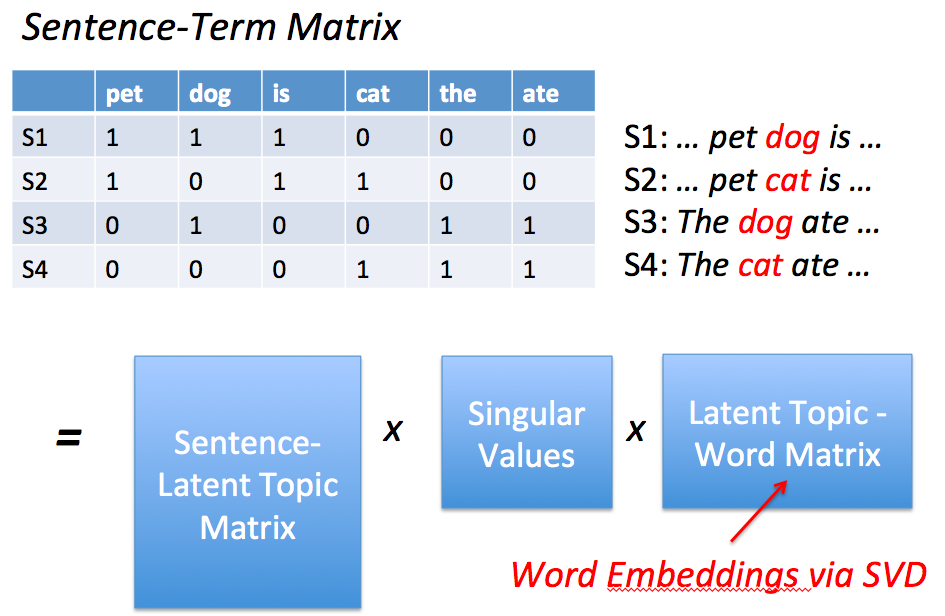
\includegraphics[width=0.9\textwidth]{figs/word_embedding_lsa}
\end{center}
\end{figure}
\end{frame}

%%% subsection
\subsection[Multiview Learning]{Multiview Learning}

\begin{frame}
\frametitle{From single-view to multi-view}
\bi
\item What are other ``definitions'' of word meaning, besides distributional semantics?
\item Can we include them in the encoding of word representations?
\ei
\end{frame}

\begin{frame}
\frametitle{View 2: Relational Semantics}
\begin{figure}[htbp]
\begin{center}
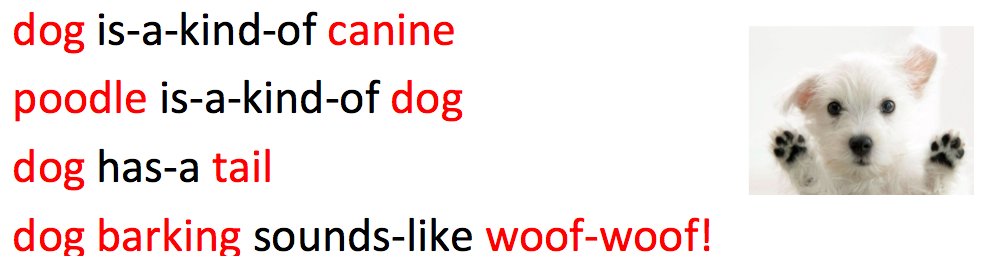
\includegraphics[width=0.9\textwidth]{figs/relational_semantics1}
\end{center}
\end{figure}
\vspace{1cm}
\bi
\item Many such relational knowledge have been created in e.g. WordNet \cite{miller95wordnet}, Freebase \cite{bollacker08freebase}
\item \cite{faruqui14retrofit,fried15iclr} incorporate both relational and distributional objectives in embeddings
\ei
\end{frame}


\begin{frame}
\frametitle{View 3: Bilingual information}
\bi
\item The translation $y$ of a word $x$ provides an additional view (different form, same meaning) 
\item Method 1: Assume word translation pairs \cite{faruqui14representation}: 
\bi
\item $v,w = CCA(x,y) = \arg\max_{v,w} \rho(xv,yw)$
\ei
\pause
\item Method 2: Assume sentence translation pairs \cite{gouws15representation}
\ei
\begin{figure}[htbp]
\begin{center}
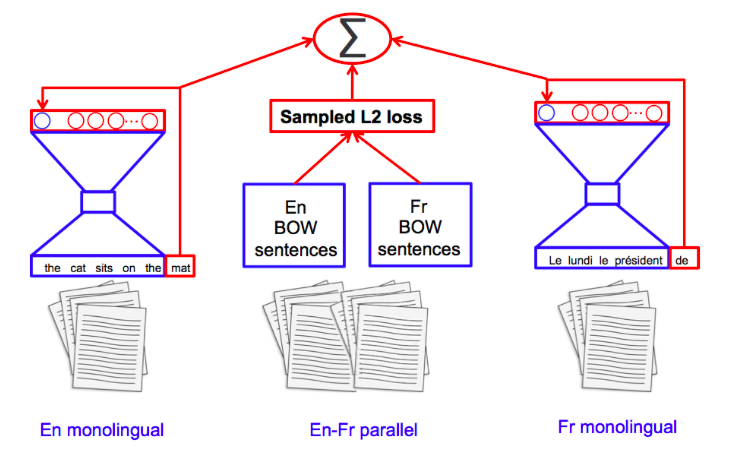
\includegraphics[width=0.6\textwidth]{figs/gouws15}
\end{center}
\end{figure}
\vspace{1cm}
\end{frame}


\begin{frame}
\frametitle{Example~\cite{faruqui14representation}}
\begin{figure}[t]
\centering
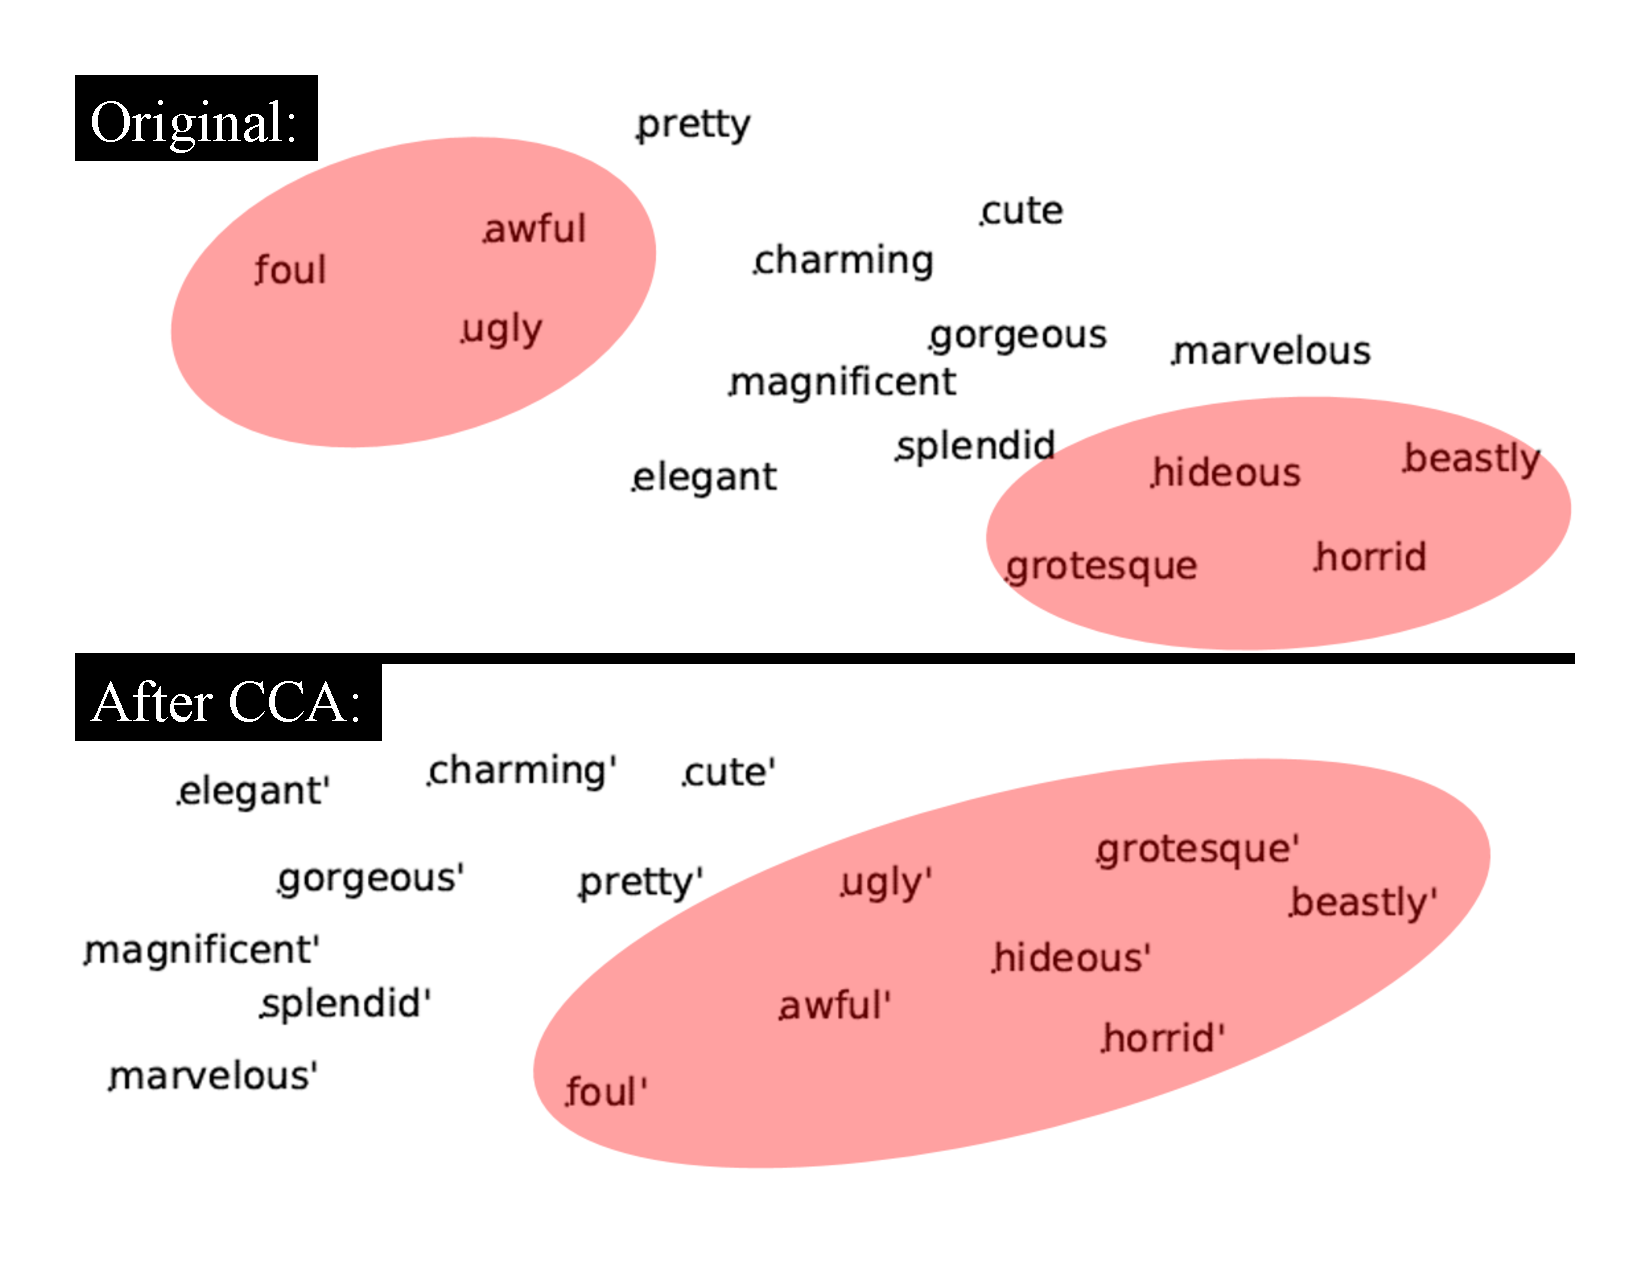
\includegraphics[width=0.7\linewidth]{figs/faruqui-dyer}
\end{figure}
Antonyms are mixed up when relying only on one language's distributional semantics (view 1), but is nicely teased apart with multilingual views.
\end{frame}


\begin{frame}
\frametitle{2+ views \cite{rastogi15multiview}}
\begin{figure}[htbp]
\begin{center}
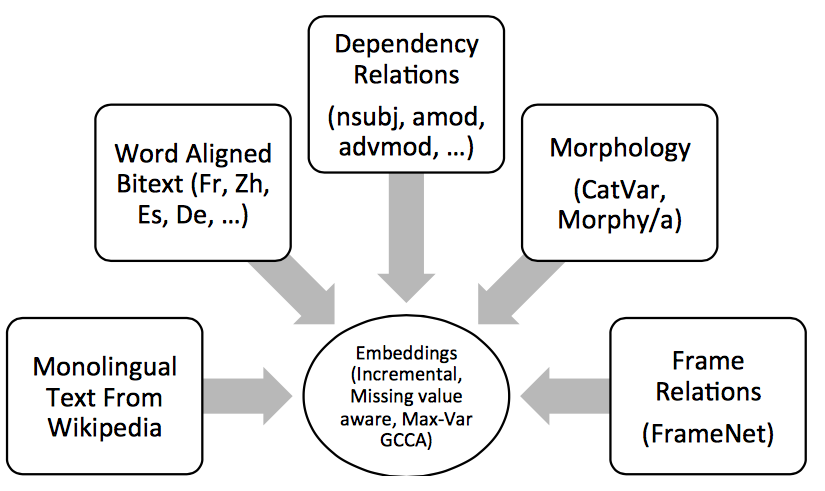
\includegraphics[width=0.6\textwidth]{figs/rastogi15a}\\
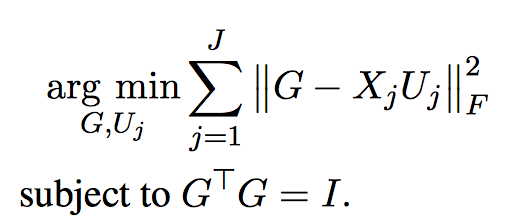
\includegraphics[width=0.6\textwidth]{figs/rastogi15b}
\end{center}
\end{figure}
\end{frame}

%% SECTION%%%%%
\section[Sentence Embedding]{Sentence Embeddings}

\subsection[What should be encoded]{What should be encoded?}

\begin{frame}
\frametitle{Challenges}
\be
\item What to encode in the representation?
\item How to handle variable length sequences?
\ee
\end{frame}


\begin{frame}
\frametitle{What should be encoded? (1) Semantic equivalence}
\bi
\item "Bob gave Jane a book on her birthday"\\\hspace{1cm}$\rightarrow$ vector ${\bf s_1}$
\item "Jane's birthday present from Bob was a book"\\\hspace{1cm} $\rightarrow$ vector ${\bf s_2}$
\item Hopefully ${\bf s_1}  = {\bf s_2}$
\pause
\vspace{0.6cm}
\item "Bob gave Jane a book on her birthday"\\\hspace{1cm}$\rightarrow$ vector ${\bf s_1}$
\item "Bob gab Jane ein Buch an ihren Geburstag"\\\hspace{1cm} $\rightarrow$ vector ${\bf s_3}$
\item Hopefully ${\bf s_1}  = {\bf s_3}$
\ei
\end{frame}

\begin{frame}
\frametitle{What should be encoded? (2) Entailment, Relatedness, and Inference}
\bi
\item s1: A sea turtle is hunting for fish
\item s2: A sea turtle is hunting for food
\item s3: The turtle is following the fish
\item s4: The turtle is following the red fish
\ei
 Does s1 entail s2? Are they semantically equivalent?\\[0.2cm]
 Does s1 entail s3? Or can you infer s3 is likely true given s1? \\[0.2cm]
\end{frame}

\begin{frame}
\frametitle{What should be encoded? (2) Entailment, Relatedness, and Inference}
\bi
\item s5: The first settlements on the site of Jakarta were established at the mouth of the Ciliwung, perhaps as early as the 5th century AD.
\item s6: The first settlements on the site of Jakarta were established as early as the 5th century AD.
\item s7: The first settlements on the site of Jakarta were established as late as the 4th century AD.
\ei 
 s6 summarizes s5. How should the vectors relate mathematically?\\[0.2cm]
 s6 and s7 are syntactically similar, but contradictory. What should be their vectors? \\[0.2cm]
\end{frame}

\begin{frame}
\frametitle{What should be encoded? (2) Entailment, Relatedness, and Inference}
\bi
\item s7: Tom was accidentally shot by his teammate in the Army
\item s8: Tom dies
\item s9: Tom is bleeding
\ei
 s8 is a possible consequence of s7 by inference. How should the vectors relate? \\[0.2cm]
 s9 is an even more likely consequence of s7 by inference. How do the three vectors relate?
\end{frame}


\begin{frame}
\frametitle{The cynic}
Does it even make sense to represent one sentence as one vector? \\[0.2cm]
One possible work-around: attention
\bi
\item Representation is $\sum_i \alpha_i v_i$ where $ 0 \leq \alpha_i \leq 1, v_i \in \mathbb{R}^d$
\item Integrate representation in an end-to-end system, and $\alpha_i$ is adaptively re-computed based on some state
\ei
\end{frame}


%%%
\begin{frame}
\frametitle{Attention in machine translation \cite{bahdanau14translate}}
\bi
\item It seems too much to expect one vector encoding of input $\bf{c}$ can do everything\pause
\item Idea: During decoding, dynamically {\color{red} pay attention} to different parts of the input.
\ei
\pause
\centerline{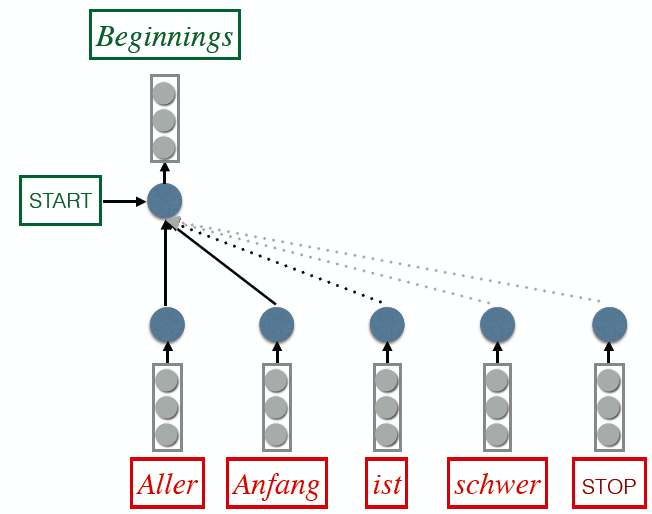
\includegraphics[scale=0.33]{figs/explain_attention1}}
\end{frame}

%%%
\begin{frame}
\frametitle{Attention in machine translation \cite{bahdanau14translate}}
\bi
\item It seems too much to expect one vector encoding of input $\bf{c}$ can do everything
\item Idea: During decoding, dynamically {\color{red} pay attention} to different parts of the input.
\ei
\centerline{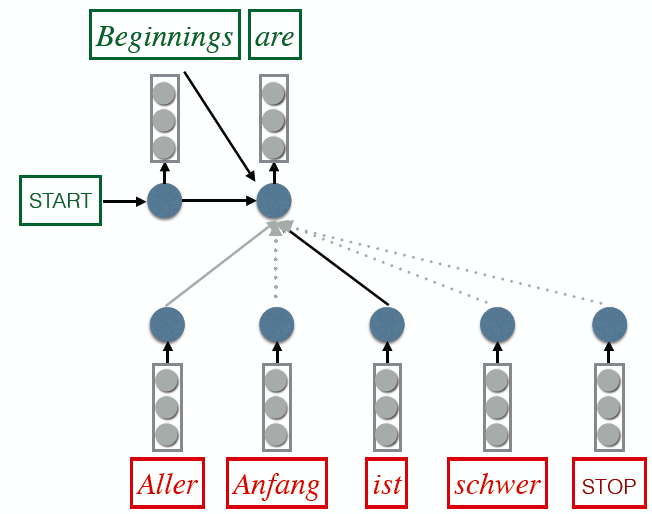
\includegraphics[scale=0.33]{figs/explain_attention2}}
\end{frame}

%%%
\begin{frame}
\frametitle{Attention in machine translation \cite{bahdanau14translate}}
\bi
\item It seems too much to expect one vector encoding of input $\bf{c}$ can do everything
\item Idea: During decoding, dynamically {\color{red} pay attention} to different parts of the input.
\ei
\centerline{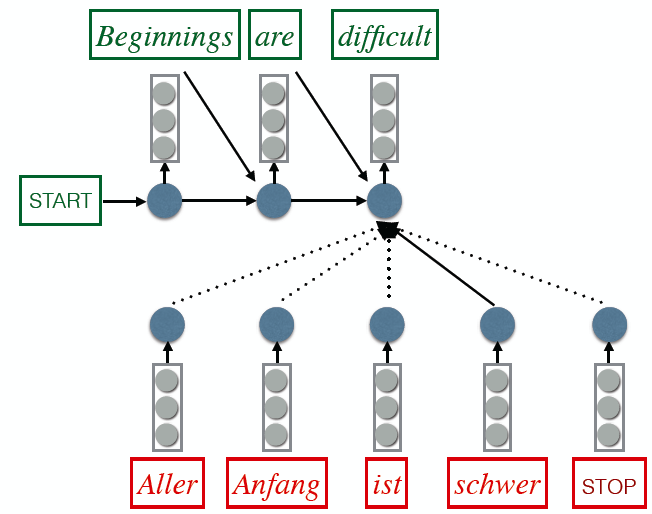
\includegraphics[scale=0.33]{figs/explain_attention3}}
\end{frame}

%%%
\begin{frame}
\frametitle{Attention in machine translation \cite{bahdanau14translate}}
\bi
\item It seems too much to expect one vector encoding of input $\bf{c}$ can do everything
\item Idea: During decoding, dynamically {\color{red} pay attention} to different parts of the input.
\ei
\centerline{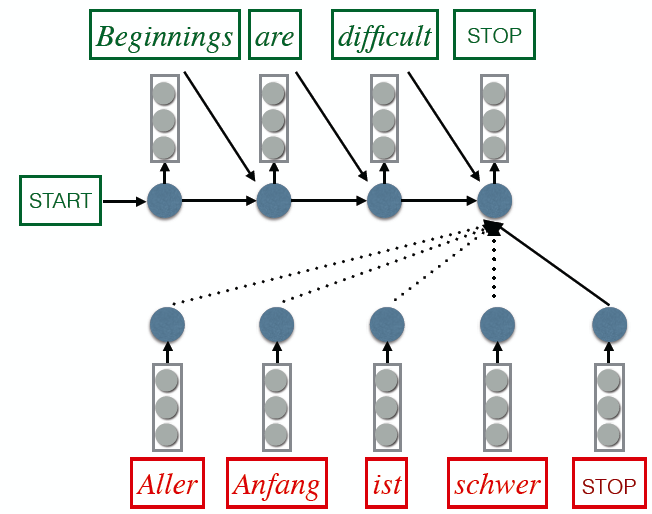
\includegraphics[scale=0.33]{figs/explain_attention4}}
\end{frame}

\subsection[Handling variable length sequences]{Handling variable length sequences}


\begin{frame}
\frametitle{Approach 1: Bag of words}
\bi
\item Sentence vector = sum of word vectors 
\item  ${\bf s} = w(Bob) + w(gave) + w(Jane) + w(a) + w(book) + w(on) + w(her) + w(birthday)$
\item Variants: product, weighted sum, bag of bigrams, ...
\ei
\end{frame}


\begin{frame}
\frametitle{Approach 2: Convolution and Recurrent units}
\bi
\item Encode variable-length sequence into fix-length vector
\centerline{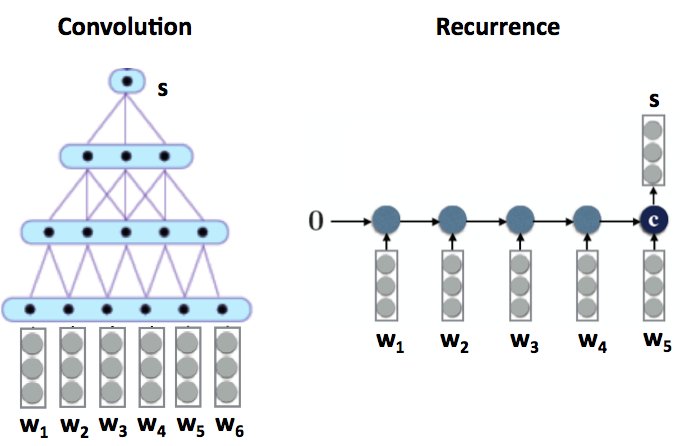
\includegraphics[scale=0.3]{figs/sentence_models_conv_recur}}
\item Examples in sentence translation \cite{kalchbrenner13,sutskevar14sequence}
\ei
\end{frame}

\begin{frame}
\frametitle{Recurrent Neural Net Language Models}
Model $p(current\_word|previous\_words)$ with a recurrent hidden layer \cite{mikolov10rnnlm}

\begin{columns}
\column{0.6\textwidth}
\scalebox{0.6}{\begin{tikzpicture}[->,>=stealth',shorten >=1pt,auto,node distance=3cm,
  thick,main node/.style={circle,fill=blue!20,draw,font=\sffamily\Large\bfseries}]

  \node[main node] (x1) at (0,0) {$x_1$};
  \node[main node] (x2) at (2,0) {$x_2$};
  \node[main node] (x3) at (4,0) {$x_3$};
  \node[main node] (x4) at (6,0) {$x_4$};
  \node[main node] (x5) at (8,0) {$x_5$};
  \node[main node] (h1) at (4,2) {$h_1$};
  \node[main node] (h2) at (6,2) {$h_2$};
  \node[main node] (h'1) at (0,4) {$y_1$};
  \node[main node] (h'2) at (2,4) {$y_2$};
  \node[main node] (h'3) at (4,4) {$y_3$};

  \draw[blue,ultra thick,-latex,<->] (0,-1) -- node[]{Previous Word} (4,-1);
  \draw[blue,ultra thick,-latex,<->] (6,-1) -- node[]{Previous $h$} (8,-1);
  \draw[blue,ultra thick,-latex,<->] (0,5) -- node[]{Current Word (assume 3-word vocabulary)} (4,5);

   \node(wij) at (1,1) {$w_{ij}$};
   \node(wjk) at (1,3) {$w_{jk}$};

  \path[every node/.style={font=\sffamily\small}]
    (x1) edge node {} (h1)
    (x2) edge node {} (h1)
    (x3) edge node {} (h1)
    (x4) edge node {} (h1)
    (x5) edge node {} (h1)
    (x1) edge node {} (h2)
    (x2) edge node {} (h2)
    (x3) edge node {} (h2)
    (x4) edge node {} (h2)
    (x5) edge node {} (h2)
    (h1) edge node {} (h'1)
    (h2) edge node {} (h'1)
    (h1) edge node {} (h'2)
    (h2) edge node {} (h'2)
    (h1) edge node {} (h'3)
    (h2) edge node {} (h'3)
    ;
\end{tikzpicture}}
    \column{.4\textwidth}
\bi
\item Probability of word: $y_k=\frac{\exp(W_{jk}^T h)}{\sum_{k'}\exp(W_{jk'}^T h)}$
\item $[x_4,x_5]$ is a copy of $[h_1,h_2]$ from the previous time-step
\item $h_j=\sigma(W_{ij}^T x_i)$ is hidden state of partial sentence
\item Arbitrarily-long history is (theoretically) kept through recurrence
\ei
\end{columns}
\end{frame}

\begin{frame}
\frametitle{Training: Backpropagation through Time}
Unroll the hidden states for a few time-steps, then backprop.\\
{\color{red} Very deep network: vanishing/exploding gradients!}

\scalebox{0.8}{\begin{tikzpicture}[->,>=stealth',shorten >=1pt,auto,node distance=3cm,
  thick,main node/.style={circle,fill=blue!20,draw,font=\sffamily\Large\bfseries}]

  \node[main node] (x1) at (0,0) {$x_1$};
  \node[main node] (x2) at (2,0) {$x_2$};
  \node[main node] (x3) at (4,0) {$x_3$};
  \node[main node] (x4) at (6,0) {$h'_1$};
  \node[main node] (x5) at (8,0) {$h'_2$};
  \node[main node] (h1) at (4,2) {$h_1$};
  \node[main node] (h2) at (6,2) {$h_2$};
  \node[main node] (h'1) at (0,4) {$y_1$};
  \node[main node] (h'2) at (2,4) {$y_2$};
  \node[main node] (h'3) at (4,4) {$y_3$};

  \node[main node] (px1) at (2,-3) {$x_1$};
  \node[main node] (px2) at (4,-3) {$x_2$};
  \node[main node] (px3) at (6,-3) {$x_3$};
  \node[main node] (px4) at (8,-3) {$h''_1$};
  \node[main node] (px5) at (10,-3) {$h''_2$};

  \draw[blue,ultra thick,-latex,<->] (2,-4) -- node[]{"Input0" $[x_1,x_2,x_3]=[0,1,0]$} (6,-4);
  \draw[blue,ultra thick,-latex,<->] (0,-1) -- node[]{"Input1" $[x_1,x_2,x_3]=[1,0,0]$} (4,-1);
 \draw[blue,ultra thick,-latex,<->] (6,-1) -- node[]{Previous $h$} (8,-1);
\draw[blue,ultra thick,-latex,<->] (8,-4) -- node[]{Initial $h$} (10,-4);
   \node(wij) at (1,1) {$w_{ij}$};
   \node(wjk) at (1,3) {$w_{jk}$};
      \node(wij) at (3,-2) {$w_{ij}$};

  \path[every node/.style={font=\sffamily\small}]
    (px1) edge node {} (x4)
    (px2) edge node {} (x4)
    (px3) edge node {} (x4)
    (px4) edge node {} (x4)
    (px5) edge node {} (x4)
    (px1) edge node {} (x5)
    (px2) edge node {} (x5)
    (px3) edge node {} (x5)
    (px4) edge node {} (x5)
    (px5) edge node {} (x5)
    (x1) edge node {} (h1)
    (x2) edge node {} (h1)
    (x3) edge node {} (h1)
    (x4) edge node {} (h1)
    (x5) edge node {} (h1)
    (x1) edge node {} (h2)
    (x2) edge node {} (h2)
    (x3) edge node {} (h2)
    (x4) edge node {} (h2)
    (x5) edge node {} (h2)
    (h1) edge node {} (h'1)
    (h2) edge node {} (h'1)
    (h1) edge node {} (h'2)
    (h2) edge node {} (h'2)
    (h1) edge node {} (h'3)
    (h2) edge node {} (h'3)
    ;
\end{tikzpicture}}
\end{frame}

%%%%%%%
\begin{frame}
\frametitle{A popular recurrent unit: LSTM}
Long Short-term Memory (LSTM): 
\bi
\item Idea: Shouldn't need to back-prop to beginning of history. Just keep a memory of important bits. \pause
\item Introduces memory cell ($c_t$), with input/output/forget gates to keep track of what to remember and when
\ei
\centerline{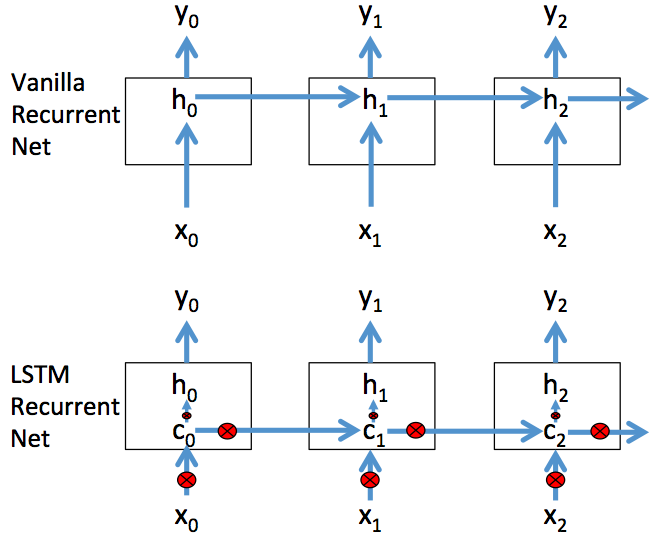
\includegraphics[scale=0.28]{figs/lstm_simpleschematic}}
\blfootnote{*Nice explanation of LSTM and variants here: \url{http://colah.github.io/posts/2015-08-Understanding-LSTMs/}}
\end{frame}

%%% 
\begin{frame}
\frametitle{LSTM in detail \cite{gers02peephole}}

\centerline{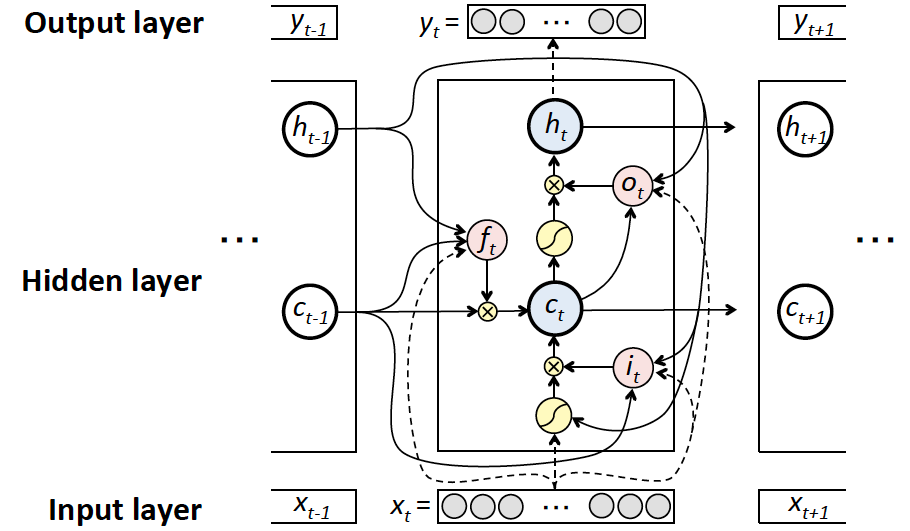
\includegraphics[scale=0.28]{figs/lstm_detailschematic}}
\vspace{-0.4cm}
\begin{eqnarray*}
  i_{t} &=&  \sigma (W_{xi} x_{t} + W_{ci} c_{t-1} + W_{hi} h_{t-1}) \\[-.25em]
  f_{t} &=&  \sigma (W_{xf} x_{t} + W_{cf} c_{t-1} + W_{hf} h_{t-1}) \\[-.25em]
  c_{t} &=&  f_{t} c_{t-1} + \!i_{t} \ tanh (W_{xc} x_{t} + W_{hc} h_{t-1}) \\[-.25em]
  o_{t} &=&  \sigma (W_{xo} x_{t} + W_{co} c_{t} + W_{ho} h_{t-1}) \\[-.25em]
  h_{t} &=&  o_{t} \tanh(c_{t}), \hspace{0.3cm}  y_{t} =  softmax(W_{hy} h_{t})
\end{eqnarray*}
\vspace{-0.2cm}
\blfootnote{Figure courtesy of Adhi Kuncoro \& Yuichiro Sawai}

\end{frame}


\begin{frame}
\frametitle{Convolution} % frame1
\begin{tikzpicture}[->,>=stealth',shorten >=1pt,auto,node distance=3cm,
  thick,main node/.style={circle,fill=blue!20,draw,font=\sffamily\Large\bfseries}]

  \node[main node] (x1) at (0,0) {$x_1$};
  \node[main node] (x2) at (2,0) {$x_2$};
  \node[main node] (x3) at (4,0) {$x_3$};
  \node[main node] (x4) at (6,0) {$x_4$};
  \node[main node] (x5) at (8,0) {$x_5$};
  \node[main node] (h1) at (2,2) {$h_1$};
  \node[main node] (h2) at (4,2) {$h_2$};
  \node[main node] (h3) at (6,2) {$h_3$};
  	
     \path[red,every node/.style={font=\sffamily\small}]
    (x1) edge node {} (h1)     ;
     \path[blue,every node/.style={font=\sffamily\small}]
    (x2) edge node {} (h1)     ;
   \path[yellow,every node/.style={font=\sffamily\small}]
    (x3) edge node {} (h1)     ;

\end{tikzpicture}
Sliding window of shared weights: $h_j = \sum_{\tau=0}^{2}w_{\tau}x_{j+\tau}$\\[0.2cm]
\end{frame}

%%%%%%%%%
\begin{frame}
\frametitle{Convolution} %frame2
\begin{tikzpicture}[->,>=stealth',shorten >=1pt,auto,node distance=3cm,
  thick,main node/.style={circle,fill=blue!20,draw,font=\sffamily\Large\bfseries}]

  \node[main node] (x1) at (0,0) {$x_1$};
  \node[main node] (x2) at (2,0) {$x_2$};
  \node[main node] (x3) at (4,0) {$x_3$};
  \node[main node] (x4) at (6,0) {$x_4$};
  \node[main node] (x5) at (8,0) {$x_5$};
  \node[main node] (h1) at (2,2) {$h_1$};
  \node[main node] (h2) at (4,2) {$h_2$};
  \node[main node] (h3) at (6,2) {$h_3$};
  
	
     \path[red,every node/.style={font=\sffamily\small}]
    (x2) edge node {} (h2)     ;
     \path[blue,every node/.style={font=\sffamily\small}]
    (x3) edge node {} (h2)     ;
   \path[yellow,every node/.style={font=\sffamily\small}]
    (x4) edge node {} (h2)     ;

\end{tikzpicture}
Sliding window of shared weights: $h_j = \sum_{\tau=0}^{2}w_{\tau}x_{j+\tau}$\\[0.2cm]
\end{frame}

%%%%%%%%%
\begin{frame}
\frametitle{Convolution} %frame3
\begin{tikzpicture}[->,>=stealth',shorten >=1pt,auto,node distance=3cm,
  thick,main node/.style={circle,fill=blue!20,draw,font=\sffamily\Large\bfseries}]

  \node[main node] (x1) at (0,0) {$x_1$};
  \node[main node] (x2) at (2,0) {$x_2$};
  \node[main node] (x3) at (4,0) {$x_3$};
  \node[main node] (x4) at (6,0) {$x_4$};
  \node[main node] (x5) at (8,0) {$x_5$};
  \node[main node] (h1) at (2,2) {$h_1$};
  \node[main node] (h2) at (4,2) {$h_2$};
  \node[main node] (h3) at (6,2) {$h_3$};
 	
     \path[red,every node/.style={font=\sffamily\small}]
    (x3) edge node {} (h3)     ;
     \path[blue,every node/.style={font=\sffamily\small}]
    (x4) edge node {} (h3)     ;
   \path[yellow,every node/.style={font=\sffamily\small}]
    (x5) edge node {} (h3)     ;

\end{tikzpicture}
Sliding window of shared weights: $h_j = \sum_{\tau=0}^{2}w_{\tau}x_{j+\tau}$\\[0.2cm]
\end{frame}

\begin{frame}
\frametitle{Convolution} % frame4
\begin{tikzpicture}[->,>=stealth',shorten >=1pt,auto,node distance=3cm,
  thick,main node/.style={circle,fill=blue!20,draw,font=\sffamily\Large\bfseries}]

  \node[main node] (x1) at (0,0) {$x_1$};
  \node[main node] (x2) at (2,0) {$x_2$};
  \node[main node] (x3) at (4,0) {$x_3$};
  \node[main node] (x4) at (6,0) {$x_4$};
  \node[main node] (x5) at (8,0) {$x_5$};
  \node[main node] (h1) at (2,2) {$h_1$};
  \node[main node] (h2) at (4,2) {$h_2$};
  \node[main node] (h3) at (6,2) {$h_3$};
  	
     \path[red,every node/.style={font=\sffamily\small}]
       (x1) edge node {} (h1)     
        (x2) edge node {} (h2)     
        (x3) edge node {} (h3)     ;

     \path[blue,every node/.style={font=\sffamily\small}]
       (x2) edge node {} (h1)     
        (x3) edge node {} (h2)     
        (x4) edge node {} (h3)     ;

   \path[yellow,every node/.style={font=\sffamily\small}]
      (x3) edge node {} (h1)     
       (x4) edge node {} (h2)     
       (x5) edge node {} (h3)     ;
\end{tikzpicture}
Sliding window of shared weights: $h_j = \sum_{\tau=0}^{2}w_{\tau}x_{j+\tau}$\\[0.2cm]
\end{frame}

\begin{frame}
\frametitle{Pooling} 
\begin{tikzpicture}[->,>=stealth',shorten >=1pt,auto,node distance=3cm,
  thick,main node/.style={circle,fill=blue!20,draw,font=\sffamily\Large\bfseries}]

  \node[main node] (x1) at (0,0) {$x_1$};
  \node[main node] (x2) at (2,0) {$x_2$};
  \node[main node] (x3) at (4,0) {$x_3$};
  \node[main node] (x4) at (6,0) {$x_4$};
  \node[main node] (x5) at (8,0) {$x_5$};
  \node[main node] (h1) at (2,2) {$h_1$};
  \node[main node] (h2) at (4,2) {$h_2$};
  \node[main node] (h3) at (6,2) {$h_3$};
  \node[main node] (p1) at (3,4) {$p_1$};
  \node[main node] (p2) at (5,4) {$p_2$};
  	
     \path[red,every node/.style={font=\sffamily\small}]
       (x1) edge node {} (h1)     
        (x2) edge node {} (h2)     
        (x3) edge node {} (h3)     ;

     \path[blue,every node/.style={font=\sffamily\small}]
       (x2) edge node {} (h1)     
        (x3) edge node {} (h2)     
        (x4) edge node {} (h3)     ;

   \path[yellow,every node/.style={font=\sffamily\small}]
      (x3) edge node {} (h1)     
       (x4) edge node {} (h2)     
       (x5) edge node {} (h3)     ;
     
     \path[every node/.style={font=\sffamily\small}]
       (h1) edge node {} (p1)     
        (h2) edge node {} (p1)     
        (h2) edge node {} (p2)  
        (h3) edge node {} (p2)    ;  
       
\end{tikzpicture}
Max-Pooling nodes: $p_1=max(h_1,h_2)$, $p_2=max(h_2,h_3)$\\[0.2cm]
Advantages of Convolution + Pooling:
\be
\item Fewer weights
\item Shift invariance
\ee
\end{frame}

\begin{frame}
\frametitle{Convolutional Nets in vision \cite{lecun98conv}}
\vspace{0.1cm}
\begin{columns}[c]
    \column{.5\textwidth}
\scalebox{0.55}{\begin{tikzpicture}[->,>=stealth',shorten >=1pt,auto,node distance=3cm,
  thick,main node/.style={circle,fill=blue!20,draw,font=\sffamily\Large\bfseries}]

  \node[main node] (x1) at (0,0) {$x_1$};
  \node[main node] (x2) at (2,0) {$x_2$};
  \node[main node] (x3) at (4,0) {$x_3$};
  \node[main node] (x4) at (6,0) {$x_4$};
  \node[main node] (x5) at (8,0) {$x_5$};
  \node[main node] (h1) at (2,2) {$h_1$};
  \node[main node] (h2) at (4,2) {$h_2$};
  \node[main node] (h3) at (6,2) {$h_3$};
  \node[main node] (h'1) at (3,4) {$p_1$};
  \node[main node] (h'2) at (5,4) {$p_2$};

  \path[every node/.style={font=\sffamily\small}]
    (x1) edge node {} (h1)
    (x2) edge node {} (h1)
    (x3) edge node {} (h1)
    (x2) edge node {} (h2)
    (x3) edge node {} (h2)
    (x4) edge node {} (h2)
    (x3) edge node {} (h3)
    (x4) edge node {} (h3)
    (x5) edge node {} (h3)
    (h1) edge node {} (h'1)
    (h2) edge node {} (h'1)
    (h2) edge node {} (h'2)
    (h3) edge node {} (h'2)
    ;
\end{tikzpicture}}
    \column{.5\textwidth}
{\bf Receptive Field (RF)}: each $h_j$ only connects to small input region via convolution.\\
{\bf Pooling}: e.g. $p_1=max(h_1,h_2)$ or $p_1=\sqrt{h_1^2+h_2^2}$\\[0.2cm]
\end{columns}
\pause
\begin{center}
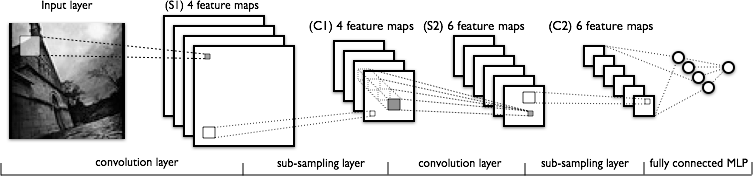
\includegraphics[scale=0.53]{figs/lenet}\\
\tiny{(Figure from \url{http://deeplearning.net/tutorial/lenet.html})}
\end{center}
\end{frame}


	



\begin{frame}
\frametitle{Summary and Thoughts}
\be
\item Word representations: 
	\bi
	\item Distributional semantics, relational semantics, etc. $\rightarrow$ multiple views we want to encode
	\item Feed-forward neural language models and word2vec
	\ei
	\pause
\item Sentence representations:
	\bi
	\item Big challenge in what to encode
	\item Technical challenge: Handling variable-length sequences. Current solutions: convolution, recurrent nets 
	\ei 
	\pause
\item Questions for you:
\bi
	\item Should there be multiple representations per word? 
		\bi
		\item "I went to see the {\em play} at the theater"; "I went to {\em play} in the park"; "That was a great {\em play} by the goal keeper."
		\ei
	\pause
	\item Do you think sentence representations should be learned bottom-up (e.g. convolution) or left-to-right (e.g. LSTM)?
	\pause
	\item What is the verdict on end-to-end learning vs. pre-trained word/sentence embeddings?
\ei
\ee
\end{frame}




%%%%%%%%%%%%%%%%%%%%
\begin{frame}[allowframebreaks]
%\frametitle{References}
\begin{tiny}
References:
\bibliographystyle{apalike}
\bibliography{mybib}
\end{tiny}
\end{frame}

\end{document}
